% Created by tikzDevice version 0.8.1 on 2015-02-19 05:31:36
% !TEX encoding = UTF-8 Unicode
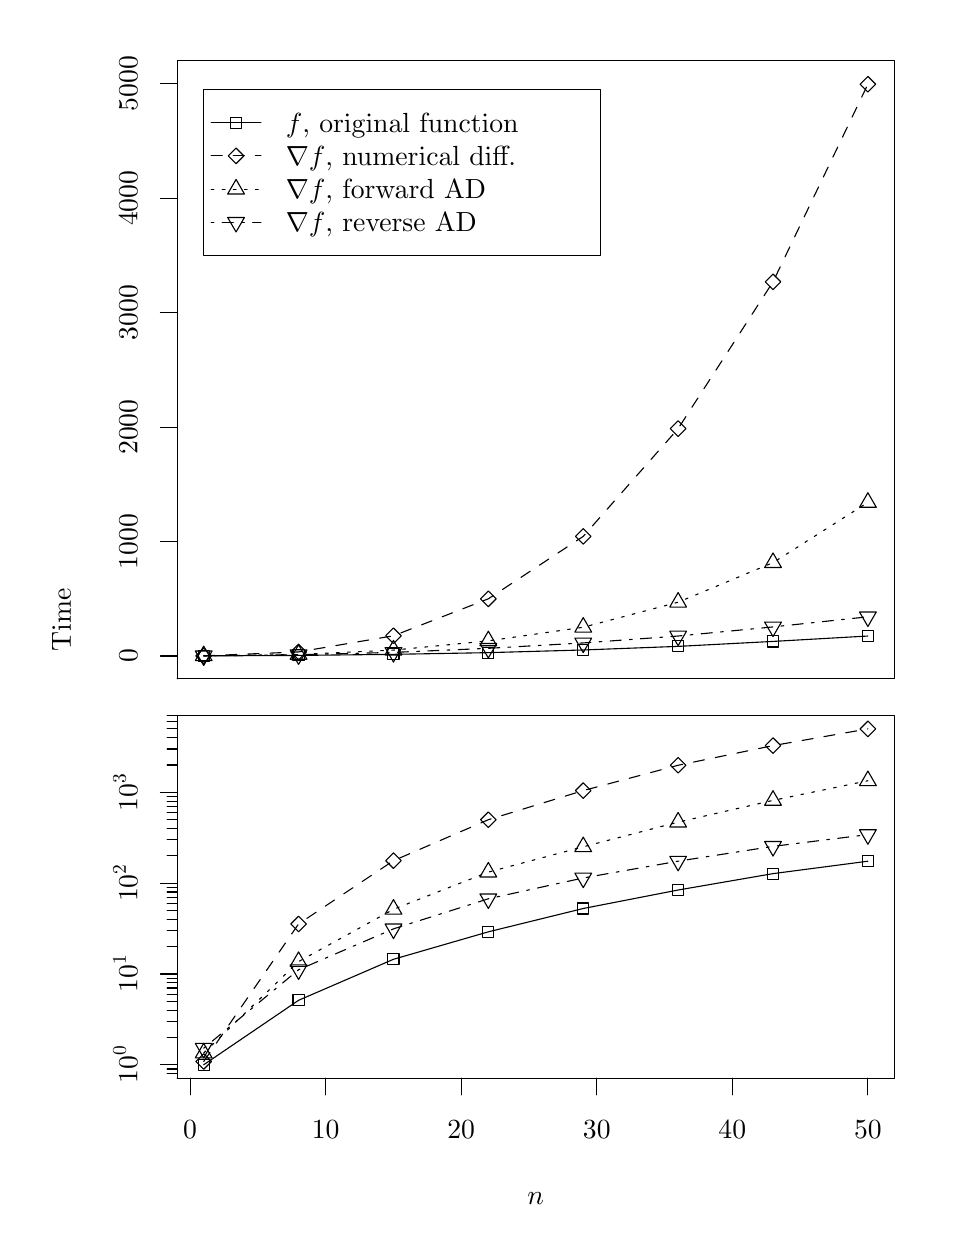
\begin{tikzpicture}[x=1pt,y=1pt]
\definecolor{fillColor}{RGB}{255,255,255}
\path[use as bounding box,fill=fillColor,fill opacity=0.00] (0,0) rectangle (325.21,433.62);
\begin{scope}
\path[clip] ( 54.00,198.30) rectangle (313.21,421.62);
\definecolor{drawColor}{RGB}{0,0,0}

\path[draw=drawColor,line width= 0.4pt,line join=round,line cap=round] ( 63.60,206.61) --
	( 97.89,206.78) --
	(132.18,207.17) --
	(166.46,207.78) --
	(200.75,208.75) --
	(235.04,210.05) --
	(269.33,211.84) --
	(303.61,213.79);

\path[draw=drawColor,line width= 0.4pt,line join=round,line cap=round] ( 61.61,204.62) rectangle ( 65.59,208.61);

\path[draw=drawColor,line width= 0.4pt,line join=round,line cap=round] ( 95.89,204.79) rectangle ( 99.88,208.78);

\path[draw=drawColor,line width= 0.4pt,line join=round,line cap=round] (130.18,205.18) rectangle (134.17,209.17);

\path[draw=drawColor,line width= 0.4pt,line join=round,line cap=round] (164.47,205.78) rectangle (168.46,209.77);

\path[draw=drawColor,line width= 0.4pt,line join=round,line cap=round] (198.76,206.75) rectangle (202.75,210.74);

\path[draw=drawColor,line width= 0.4pt,line join=round,line cap=round] (233.05,208.05) rectangle (237.03,212.04);

\path[draw=drawColor,line width= 0.4pt,line join=round,line cap=round] (267.33,209.84) rectangle (271.32,213.83);

\path[draw=drawColor,line width= 0.4pt,line join=round,line cap=round] (301.62,211.79) rectangle (305.61,215.78);
\end{scope}
\begin{scope}
\path[clip] (  0.00,  0.00) rectangle (325.21,433.62);
\definecolor{drawColor}{RGB}{0,0,0}

\path[draw=drawColor,line width= 0.4pt,line join=round,line cap=round] ( 54.00,206.57) -- ( 54.00,413.35);

\path[draw=drawColor,line width= 0.4pt,line join=round,line cap=round] ( 54.00,206.57) -- ( 48.00,206.57);

\path[draw=drawColor,line width= 0.4pt,line join=round,line cap=round] ( 54.00,247.93) -- ( 48.00,247.93);

\path[draw=drawColor,line width= 0.4pt,line join=round,line cap=round] ( 54.00,289.28) -- ( 48.00,289.28);

\path[draw=drawColor,line width= 0.4pt,line join=round,line cap=round] ( 54.00,330.64) -- ( 48.00,330.64);

\path[draw=drawColor,line width= 0.4pt,line join=round,line cap=round] ( 54.00,371.99) -- ( 48.00,371.99);

\path[draw=drawColor,line width= 0.4pt,line join=round,line cap=round] ( 54.00,413.35) -- ( 48.00,413.35);

\node[text=drawColor,rotate= 90.00,anchor=base,inner sep=0pt, outer sep=0pt, scale=  1.00] at ( 39.60,206.57) {0};

\node[text=drawColor,rotate= 90.00,anchor=base,inner sep=0pt, outer sep=0pt, scale=  1.00] at ( 39.60,247.93) {1000};

\node[text=drawColor,rotate= 90.00,anchor=base,inner sep=0pt, outer sep=0pt, scale=  1.00] at ( 39.60,289.28) {2000};

\node[text=drawColor,rotate= 90.00,anchor=base,inner sep=0pt, outer sep=0pt, scale=  1.00] at ( 39.60,330.64) {3000};

\node[text=drawColor,rotate= 90.00,anchor=base,inner sep=0pt, outer sep=0pt, scale=  1.00] at ( 39.60,371.99) {4000};

\node[text=drawColor,rotate= 90.00,anchor=base,inner sep=0pt, outer sep=0pt, scale=  1.00] at ( 39.60,413.35) {5000};

\path[draw=drawColor,line width= 0.4pt,line join=round,line cap=round] ( 54.00,198.30) --
	(313.21,198.30) --
	(313.21,421.62) --
	( 54.00,421.62) --
	( 54.00,198.30);
\end{scope}
\begin{scope}
\path[clip] ( 54.00,198.30) rectangle (313.21,421.62);
\definecolor{drawColor}{RGB}{0,0,0}

\path[draw=drawColor,line width= 0.4pt,dash pattern=on 4pt off 4pt ,line join=round,line cap=round] ( 63.60,206.62) --
	( 97.89,208.04) --
	(132.18,213.88) --
	(166.46,227.23) --
	(200.75,249.80) --
	(235.04,288.73) --
	(269.33,341.78) --
	(303.61,413.18);

\path[draw=drawColor,line width= 0.4pt,line join=round,line cap=round] ( 63.60,203.80) --
	( 66.42,206.62) --
	( 63.60,209.44) --
	( 60.78,206.62) --
	( 63.60,203.80);

\path[draw=drawColor,line width= 0.4pt,line join=round,line cap=round] ( 97.89,205.22) --
	(100.71,208.04) --
	( 97.89,210.86) --
	( 95.07,208.04) --
	( 97.89,205.22);

\path[draw=drawColor,line width= 0.4pt,line join=round,line cap=round] (132.18,211.06) --
	(135.00,213.88) --
	(132.18,216.70) --
	(129.36,213.88) --
	(132.18,211.06);

\path[draw=drawColor,line width= 0.4pt,line join=round,line cap=round] (166.46,224.41) --
	(169.28,227.23) --
	(166.46,230.05) --
	(163.64,227.23) --
	(166.46,224.41);

\path[draw=drawColor,line width= 0.4pt,line join=round,line cap=round] (200.75,246.98) --
	(203.57,249.80) --
	(200.75,252.62) --
	(197.93,249.80) --
	(200.75,246.98);

\path[draw=drawColor,line width= 0.4pt,line join=round,line cap=round] (235.04,285.91) --
	(237.86,288.73) --
	(235.04,291.55) --
	(232.22,288.73) --
	(235.04,285.91);

\path[draw=drawColor,line width= 0.4pt,line join=round,line cap=round] (269.33,338.96) --
	(272.15,341.78) --
	(269.33,344.60) --
	(266.51,341.78) --
	(269.33,338.96);

\path[draw=drawColor,line width= 0.4pt,line join=round,line cap=round] (303.61,410.36) --
	(306.43,413.18) --
	(303.61,416.00) --
	(300.79,413.18) --
	(303.61,410.36);

\path[draw=drawColor,line width= 0.4pt,dash pattern=on 1pt off 3pt ,line join=round,line cap=round] ( 63.60,206.63) --
	( 97.89,207.14) --
	(132.18,208.70) --
	(166.46,212.04) --
	(200.75,216.96) --
	(235.04,226.00) --
	(269.33,240.30) --
	(303.61,262.07);

\path[draw=drawColor,line width= 0.4pt,line join=round,line cap=round] ( 63.60,210.13) --
	( 66.63,204.88) --
	( 60.57,204.88) --
	( 63.60,210.13);

\path[draw=drawColor,line width= 0.4pt,line join=round,line cap=round] ( 97.89,210.64) --
	(100.92,205.39) --
	( 94.86,205.39) --
	( 97.89,210.64);

\path[draw=drawColor,line width= 0.4pt,line join=round,line cap=round] (132.18,212.20) --
	(135.21,206.95) --
	(129.15,206.95) --
	(132.18,212.20);

\path[draw=drawColor,line width= 0.4pt,line join=round,line cap=round] (166.46,215.54) --
	(169.49,210.29) --
	(163.43,210.29) --
	(166.46,215.54);

\path[draw=drawColor,line width= 0.4pt,line join=round,line cap=round] (200.75,220.46) --
	(203.78,215.22) --
	(197.72,215.22) --
	(200.75,220.46);

\path[draw=drawColor,line width= 0.4pt,line join=round,line cap=round] (235.04,229.50) --
	(238.07,224.25) --
	(232.01,224.25) --
	(235.04,229.50);

\path[draw=drawColor,line width= 0.4pt,line join=round,line cap=round] (269.33,243.80) --
	(272.36,238.55) --
	(266.30,238.55) --
	(269.33,243.80);

\path[draw=drawColor,line width= 0.4pt,line join=round,line cap=round] (303.61,265.57) --
	(306.64,260.32) --
	(300.58,260.32) --
	(303.61,265.57);

\path[draw=drawColor,line width= 0.4pt,dash pattern=on 1pt off 3pt on 4pt off 3pt ,line join=round,line cap=round] ( 63.60,206.63) --
	( 97.89,207.03) --
	(132.18,207.87) --
	(166.46,209.35) --
	(200.75,211.29) --
	(235.04,213.79) --
	(269.33,217.08) --
	(303.61,220.73);

\path[draw=drawColor,line width= 0.4pt,line join=round,line cap=round] ( 63.60,203.14) --
	( 66.63,208.38) --
	( 60.57,208.38) --
	( 63.60,203.14);

\path[draw=drawColor,line width= 0.4pt,line join=round,line cap=round] ( 97.89,203.53) --
	(100.92,208.78) --
	( 94.86,208.78) --
	( 97.89,203.53);

\path[draw=drawColor,line width= 0.4pt,line join=round,line cap=round] (132.18,204.37) --
	(135.21,209.62) --
	(129.15,209.62) --
	(132.18,204.37);

\path[draw=drawColor,line width= 0.4pt,line join=round,line cap=round] (166.46,205.85) --
	(169.49,211.10) --
	(163.43,211.10) --
	(166.46,205.85);

\path[draw=drawColor,line width= 0.4pt,line join=round,line cap=round] (200.75,207.79) --
	(203.78,213.03) --
	(197.72,213.03) --
	(200.75,207.79);

\path[draw=drawColor,line width= 0.4pt,line join=round,line cap=round] (235.04,210.29) --
	(238.07,215.54) --
	(232.01,215.54) --
	(235.04,210.29);

\path[draw=drawColor,line width= 0.4pt,line join=round,line cap=round] (269.33,213.58) --
	(272.36,218.83) --
	(266.30,218.83) --
	(269.33,213.58);

\path[draw=drawColor,line width= 0.4pt,line join=round,line cap=round] (303.61,217.23) --
	(306.64,222.48) --
	(300.58,222.48) --
	(303.61,217.23);

\path[draw=drawColor,line width= 0.4pt,line join=round,line cap=round] ( 63.60,411.28) rectangle (207.00,351.28);

\path[draw=drawColor,line width= 0.4pt,line join=round,line cap=round] ( 66.30,399.28) -- ( 84.30,399.28);

\path[draw=drawColor,line width= 0.4pt,dash pattern=on 4pt off 4pt ,line join=round,line cap=round] ( 66.30,387.28) -- ( 84.30,387.28);

\path[draw=drawColor,line width= 0.4pt,dash pattern=on 1pt off 3pt ,line join=round,line cap=round] ( 66.30,375.28) -- ( 84.30,375.28);

\path[draw=drawColor,line width= 0.4pt,dash pattern=on 1pt off 3pt on 4pt off 3pt ,line join=round,line cap=round] ( 66.30,363.28) -- ( 84.30,363.28);

\path[draw=drawColor,line width= 0.4pt,line join=round,line cap=round] ( 73.31,397.29) rectangle ( 77.29,401.28);

\path[draw=drawColor,line width= 0.4pt,line join=round,line cap=round] ( 75.30,384.46) --
	( 78.12,387.28) --
	( 75.30,390.10) --
	( 72.48,387.28) --
	( 75.30,384.46);

\path[draw=drawColor,line width= 0.4pt,line join=round,line cap=round] ( 75.30,378.78) --
	( 78.33,373.53) --
	( 72.27,373.53) --
	( 75.30,378.78);

\path[draw=drawColor,line width= 0.4pt,line join=round,line cap=round] ( 75.30,359.78) --
	( 78.33,365.03) --
	( 72.27,365.03) --
	( 75.30,359.78);

\node[text=drawColor,anchor=base west,inner sep=0pt, outer sep=0pt, scale=  1.00] at ( 93.30,395.84) {$f$, original function};

\node[text=drawColor,anchor=base west,inner sep=0pt, outer sep=0pt, scale=  1.00] at ( 93.30,383.84) {$\nabla f$, numerical diff.};

\node[text=drawColor,anchor=base west,inner sep=0pt, outer sep=0pt, scale=  1.00] at ( 93.30,371.84) {$\nabla f$, forward AD};

\node[text=drawColor,anchor=base west,inner sep=0pt, outer sep=0pt, scale=  1.00] at ( 93.30,359.84) {$\nabla f$, reverse AD};
\end{scope}
\begin{scope}
\path[clip] ( 54.00, 54.00) rectangle (313.21,185.10);
\definecolor{drawColor}{RGB}{0,0,0}

\path[draw=drawColor,line width= 0.4pt,line join=round,line cap=round] ( 63.60, 58.86) --
	( 97.89, 82.16) --
	(132.18, 96.98) --
	(166.46,106.90) --
	(200.75,115.33) --
	(235.04,122.01) --
	(269.33,127.93) --
	(303.61,132.42);

\path[draw=drawColor,line width= 0.4pt,line join=round,line cap=round] ( 61.61, 56.86) rectangle ( 65.59, 60.85);

\path[draw=drawColor,line width= 0.4pt,line join=round,line cap=round] ( 95.89, 80.16) rectangle ( 99.88, 84.15);

\path[draw=drawColor,line width= 0.4pt,line join=round,line cap=round] (130.18, 94.99) rectangle (134.17, 98.98);

\path[draw=drawColor,line width= 0.4pt,line join=round,line cap=round] (164.47,104.91) rectangle (168.46,108.90);

\path[draw=drawColor,line width= 0.4pt,line join=round,line cap=round] (198.76,113.34) rectangle (202.75,117.32);

\path[draw=drawColor,line width= 0.4pt,line join=round,line cap=round] (233.05,120.01) rectangle (237.03,124.00);

\path[draw=drawColor,line width= 0.4pt,line join=round,line cap=round] (267.33,125.94) rectangle (271.32,129.93);

\path[draw=drawColor,line width= 0.4pt,line join=round,line cap=round] (301.62,130.43) rectangle (305.61,134.41);
\end{scope}
\begin{scope}
\path[clip] (  0.00,  0.00) rectangle (325.21,433.62);
\definecolor{drawColor}{RGB}{0,0,0}

\path[draw=drawColor,line width= 0.4pt,line join=round,line cap=round] ( 58.70, 54.00) -- (303.61, 54.00);

\path[draw=drawColor,line width= 0.4pt,line join=round,line cap=round] ( 58.70, 54.00) -- ( 58.70, 48.00);

\path[draw=drawColor,line width= 0.4pt,line join=round,line cap=round] (107.68, 54.00) -- (107.68, 48.00);

\path[draw=drawColor,line width= 0.4pt,line join=round,line cap=round] (156.67, 54.00) -- (156.67, 48.00);

\path[draw=drawColor,line width= 0.4pt,line join=round,line cap=round] (205.65, 54.00) -- (205.65, 48.00);

\path[draw=drawColor,line width= 0.4pt,line join=round,line cap=round] (254.63, 54.00) -- (254.63, 48.00);

\path[draw=drawColor,line width= 0.4pt,line join=round,line cap=round] (303.61, 54.00) -- (303.61, 48.00);

\node[text=drawColor,anchor=base,inner sep=0pt, outer sep=0pt, scale=  1.00] at ( 58.70, 32.40) {0};

\node[text=drawColor,anchor=base,inner sep=0pt, outer sep=0pt, scale=  1.00] at (107.68, 32.40) {10};

\node[text=drawColor,anchor=base,inner sep=0pt, outer sep=0pt, scale=  1.00] at (156.67, 32.40) {20};

\node[text=drawColor,anchor=base,inner sep=0pt, outer sep=0pt, scale=  1.00] at (205.65, 32.40) {30};

\node[text=drawColor,anchor=base,inner sep=0pt, outer sep=0pt, scale=  1.00] at (254.63, 32.40) {40};

\node[text=drawColor,anchor=base,inner sep=0pt, outer sep=0pt, scale=  1.00] at (303.61, 32.40) {50};

\path[draw=drawColor,line width= 0.4pt,line join=round,line cap=round] ( 54.00, 54.00) --
	(313.21, 54.00) --
	(313.21,185.10) --
	( 54.00,185.10) --
	( 54.00, 54.00);
\end{scope}
\begin{scope}
\path[clip] (  0.00,  0.00) rectangle (325.21,197.10);
\definecolor{drawColor}{RGB}{0,0,0}

\node[text=drawColor,anchor=base,inner sep=0pt, outer sep=0pt, scale=  1.00] at (183.61,  8.40) {$n$};
\end{scope}
\begin{scope}
\path[clip] (  0.00,  0.00) rectangle (325.21,433.62);
\definecolor{drawColor}{RGB}{0,0,0}

\path[draw=drawColor,line width= 0.4pt,line join=round,line cap=round] ( 54.00, 58.86) -- ( 54.00,157.31);

\path[draw=drawColor,line width= 0.4pt,line join=round,line cap=round] ( 54.00, 58.86) -- ( 48.00, 58.86);

\path[draw=drawColor,line width= 0.4pt,line join=round,line cap=round] ( 54.00, 91.67) -- ( 48.00, 91.67);

\path[draw=drawColor,line width= 0.4pt,line join=round,line cap=round] ( 54.00,124.49) -- ( 48.00,124.49);

\path[draw=drawColor,line width= 0.4pt,line join=round,line cap=round] ( 54.00,157.31) -- ( 48.00,157.31);

\node[text=drawColor,rotate= 90.00,anchor=base west,inner sep=0pt, outer sep=0pt, scale=  1.00] at ( 39.60, 52.11) {10};

\node[text=drawColor,rotate= 90.00,anchor=base west,inner sep=0pt, outer sep=0pt, scale=  0.70] at ( 35.51, 62.10) {0};

\node[text=drawColor,rotate= 90.00,anchor=base west,inner sep=0pt, outer sep=0pt, scale=  1.00] at ( 39.60, 84.92) {10};

\node[text=drawColor,rotate= 90.00,anchor=base west,inner sep=0pt, outer sep=0pt, scale=  0.70] at ( 35.51, 94.92) {1};

\node[text=drawColor,rotate= 90.00,anchor=base west,inner sep=0pt, outer sep=0pt, scale=  1.00] at ( 39.60,117.74) {10};

\node[text=drawColor,rotate= 90.00,anchor=base west,inner sep=0pt, outer sep=0pt, scale=  0.70] at ( 35.51,127.74) {2};

\node[text=drawColor,rotate= 90.00,anchor=base west,inner sep=0pt, outer sep=0pt, scale=  1.00] at ( 39.60,150.56) {10};

\node[text=drawColor,rotate= 90.00,anchor=base west,inner sep=0pt, outer sep=0pt, scale=  0.70] at ( 35.51,160.56) {3};

\path[draw=drawColor,line width= 0.4pt,line join=round,line cap=round] ( 54.00, 55.68) -- ( 54.00,185.04);

\path[draw=drawColor,line width= 0.4pt,line join=round,line cap=round] ( 54.00, 55.68) -- ( 50.40, 55.68);

\path[draw=drawColor,line width= 0.4pt,line join=round,line cap=round] ( 54.00, 57.35) -- ( 50.40, 57.35);

\path[draw=drawColor,line width= 0.4pt,line join=round,line cap=round] ( 54.00, 68.73) -- ( 50.40, 68.73);

\path[draw=drawColor,line width= 0.4pt,line join=round,line cap=round] ( 54.00, 74.51) -- ( 50.40, 74.51);

\path[draw=drawColor,line width= 0.4pt,line join=round,line cap=round] ( 54.00, 78.61) -- ( 50.40, 78.61);

\path[draw=drawColor,line width= 0.4pt,line join=round,line cap=round] ( 54.00, 81.79) -- ( 50.40, 81.79);

\path[draw=drawColor,line width= 0.4pt,line join=round,line cap=round] ( 54.00, 84.39) -- ( 50.40, 84.39);

\path[draw=drawColor,line width= 0.4pt,line join=round,line cap=round] ( 54.00, 86.59) -- ( 50.40, 86.59);

\path[draw=drawColor,line width= 0.4pt,line join=round,line cap=round] ( 54.00, 88.49) -- ( 50.40, 88.49);

\path[draw=drawColor,line width= 0.4pt,line join=round,line cap=round] ( 54.00, 90.17) -- ( 50.40, 90.17);

\path[draw=drawColor,line width= 0.4pt,line join=round,line cap=round] ( 54.00,101.55) -- ( 50.40,101.55);

\path[draw=drawColor,line width= 0.4pt,line join=round,line cap=round] ( 54.00,107.33) -- ( 50.40,107.33);

\path[draw=drawColor,line width= 0.4pt,line join=round,line cap=round] ( 54.00,111.43) -- ( 50.40,111.43);

\path[draw=drawColor,line width= 0.4pt,line join=round,line cap=round] ( 54.00,114.61) -- ( 50.40,114.61);

\path[draw=drawColor,line width= 0.4pt,line join=round,line cap=round] ( 54.00,117.21) -- ( 50.40,117.21);

\path[draw=drawColor,line width= 0.4pt,line join=round,line cap=round] ( 54.00,119.41) -- ( 50.40,119.41);

\path[draw=drawColor,line width= 0.4pt,line join=round,line cap=round] ( 54.00,121.31) -- ( 50.40,121.31);

\path[draw=drawColor,line width= 0.4pt,line join=round,line cap=round] ( 54.00,122.99) -- ( 50.40,122.99);

\path[draw=drawColor,line width= 0.4pt,line join=round,line cap=round] ( 54.00,134.37) -- ( 50.40,134.37);

\path[draw=drawColor,line width= 0.4pt,line join=round,line cap=round] ( 54.00,140.15) -- ( 50.40,140.15);

\path[draw=drawColor,line width= 0.4pt,line join=round,line cap=round] ( 54.00,144.25) -- ( 50.40,144.25);

\path[draw=drawColor,line width= 0.4pt,line join=round,line cap=round] ( 54.00,147.43) -- ( 50.40,147.43);

\path[draw=drawColor,line width= 0.4pt,line join=round,line cap=round] ( 54.00,150.03) -- ( 50.40,150.03);

\path[draw=drawColor,line width= 0.4pt,line join=round,line cap=round] ( 54.00,152.22) -- ( 50.40,152.22);

\path[draw=drawColor,line width= 0.4pt,line join=round,line cap=round] ( 54.00,154.13) -- ( 50.40,154.13);

\path[draw=drawColor,line width= 0.4pt,line join=round,line cap=round] ( 54.00,155.80) -- ( 50.40,155.80);

\path[draw=drawColor,line width= 0.4pt,line join=round,line cap=round] ( 54.00,167.19) -- ( 50.40,167.19);

\path[draw=drawColor,line width= 0.4pt,line join=round,line cap=round] ( 54.00,172.96) -- ( 50.40,172.96);

\path[draw=drawColor,line width= 0.4pt,line join=round,line cap=round] ( 54.00,177.06) -- ( 50.40,177.06);

\path[draw=drawColor,line width= 0.4pt,line join=round,line cap=round] ( 54.00,180.24) -- ( 50.40,180.24);

\path[draw=drawColor,line width= 0.4pt,line join=round,line cap=round] ( 54.00,182.84) -- ( 50.40,182.84);

\path[draw=drawColor,line width= 0.4pt,line join=round,line cap=round] ( 54.00,185.04) -- ( 50.40,185.04);
\end{scope}
\begin{scope}
\path[clip] ( 54.00, 54.00) rectangle (313.21,185.10);
\definecolor{drawColor}{RGB}{0,0,0}

\path[draw=drawColor,line width= 0.4pt,dash pattern=on 4pt off 4pt ,line join=round,line cap=round] ( 63.60, 60.04) --
	( 97.89,109.75) --
	(132.18,132.61) --
	(166.46,147.41) --
	(200.75,157.94) --
	(235.04,167.09) --
	(269.33,174.19) --
	(303.61,180.23);

\path[draw=drawColor,line width= 0.4pt,line join=round,line cap=round] ( 63.60, 57.22) --
	( 66.42, 60.04) --
	( 63.60, 62.86) --
	( 60.78, 60.04) --
	( 63.60, 57.22);

\path[draw=drawColor,line width= 0.4pt,line join=round,line cap=round] ( 97.89,106.93) --
	(100.71,109.75) --
	( 97.89,112.57) --
	( 95.07,109.75) --
	( 97.89,106.93);

\path[draw=drawColor,line width= 0.4pt,line join=round,line cap=round] (132.18,129.79) --
	(135.00,132.61) --
	(132.18,135.43) --
	(129.36,132.61) --
	(132.18,129.79);

\path[draw=drawColor,line width= 0.4pt,line join=round,line cap=round] (166.46,144.59) --
	(169.28,147.41) --
	(166.46,150.23) --
	(163.64,147.41) --
	(166.46,144.59);

\path[draw=drawColor,line width= 0.4pt,line join=round,line cap=round] (200.75,155.12) --
	(203.57,157.94) --
	(200.75,160.76) --
	(197.93,157.94) --
	(200.75,155.12);

\path[draw=drawColor,line width= 0.4pt,line join=round,line cap=round] (235.04,164.27) --
	(237.86,167.09) --
	(235.04,169.91) --
	(232.22,167.09) --
	(235.04,164.27);

\path[draw=drawColor,line width= 0.4pt,line join=round,line cap=round] (269.33,171.37) --
	(272.15,174.19) --
	(269.33,177.01) --
	(266.51,174.19) --
	(269.33,171.37);

\path[draw=drawColor,line width= 0.4pt,line join=round,line cap=round] (303.61,177.41) --
	(306.43,180.23) --
	(303.61,183.05) --
	(300.79,180.23) --
	(303.61,177.41);

\path[draw=drawColor,line width= 0.4pt,dash pattern=on 1pt off 3pt ,line join=round,line cap=round] ( 63.60, 63.11) --
	( 97.89, 96.15) --
	(132.18,115.04) --
	(166.46,128.48) --
	(200.75,137.62) --
	(235.04,146.54) --
	(269.33,154.40) --
	(303.61,161.50);

\path[draw=drawColor,line width= 0.4pt,line join=round,line cap=round] ( 63.60, 66.61) --
	( 66.63, 61.36) --
	( 60.57, 61.36) --
	( 63.60, 66.61);

\path[draw=drawColor,line width= 0.4pt,line join=round,line cap=round] ( 97.89, 99.65) --
	(100.92, 94.40) --
	( 94.86, 94.40) --
	( 97.89, 99.65);

\path[draw=drawColor,line width= 0.4pt,line join=round,line cap=round] (132.18,118.54) --
	(135.21,113.29) --
	(129.15,113.29) --
	(132.18,118.54);

\path[draw=drawColor,line width= 0.4pt,line join=round,line cap=round] (166.46,131.98) --
	(169.49,126.73) --
	(163.43,126.73) --
	(166.46,131.98);

\path[draw=drawColor,line width= 0.4pt,line join=round,line cap=round] (200.75,141.12) --
	(203.78,135.87) --
	(197.72,135.87) --
	(200.75,141.12);

\path[draw=drawColor,line width= 0.4pt,line join=round,line cap=round] (235.04,150.04) --
	(238.07,144.79) --
	(232.01,144.79) --
	(235.04,150.04);

\path[draw=drawColor,line width= 0.4pt,line join=round,line cap=round] (269.33,157.90) --
	(272.36,152.65) --
	(266.30,152.65) --
	(269.33,157.90);

\path[draw=drawColor,line width= 0.4pt,line join=round,line cap=round] (303.61,165.00) --
	(306.64,159.75) --
	(300.58,159.75) --
	(303.61,165.00);

\path[draw=drawColor,line width= 0.4pt,dash pattern=on 1pt off 3pt on 4pt off 3pt ,line join=round,line cap=round] ( 63.60, 64.84) --
	( 97.89, 93.19) --
	(132.18,107.97) --
	(166.46,118.84) --
	(200.75,126.36) --
	(235.04,132.43) --
	(269.33,137.78) --
	(303.61,142.03);

\path[draw=drawColor,line width= 0.4pt,line join=round,line cap=round] ( 63.60, 61.34) --
	( 66.63, 66.59) --
	( 60.57, 66.59) --
	( 63.60, 61.34);

\path[draw=drawColor,line width= 0.4pt,line join=round,line cap=round] ( 97.89, 89.69) --
	(100.92, 94.94) --
	( 94.86, 94.94) --
	( 97.89, 89.69);

\path[draw=drawColor,line width= 0.4pt,line join=round,line cap=round] (132.18,104.47) --
	(135.21,109.72) --
	(129.15,109.72) --
	(132.18,104.47);

\path[draw=drawColor,line width= 0.4pt,line join=round,line cap=round] (166.46,115.34) --
	(169.49,120.59) --
	(163.43,120.59) --
	(166.46,115.34);

\path[draw=drawColor,line width= 0.4pt,line join=round,line cap=round] (200.75,122.86) --
	(203.78,128.11) --
	(197.72,128.11) --
	(200.75,122.86);

\path[draw=drawColor,line width= 0.4pt,line join=round,line cap=round] (235.04,128.94) --
	(238.07,134.18) --
	(232.01,134.18) --
	(235.04,128.94);

\path[draw=drawColor,line width= 0.4pt,line join=round,line cap=round] (269.33,134.28) --
	(272.36,139.53) --
	(266.30,139.53) --
	(269.33,134.28);

\path[draw=drawColor,line width= 0.4pt,line join=round,line cap=round] (303.61,138.53) --
	(306.64,143.78) --
	(300.58,143.78) --
	(303.61,138.53);
\end{scope}
\begin{scope}
\path[clip] (  0.00,  0.00) rectangle (325.21,433.62);
\definecolor{drawColor}{RGB}{0,0,0}

\node[text=drawColor,rotate= 90.00,anchor=base,inner sep=0pt, outer sep=0pt, scale=  1.00] at ( 15.60,219.76) {Time};
\end{scope}
\end{tikzpicture}
